%==========================オプションおよび文書クラスの設定==========================
%"autodetect-engine"-どのエンジンでもコンパイル可能にするオプション
%"dvipdfmx-if-dvi"-必要な場合のみdvipdfmx経由のpdf化をするオプション(LuaTeXやXeTeXはPDFに直接変換するため)
%"ja=standard"-日本語文書の標準設定を利用するオプション
%"bxjs…"-どのエンジンでも利用可能なドキュメントクラス
%--以下のいずれかを選択--
\documentclass[autodetect-engine,dvipdfmx-if-dvi,ja=standard,a4paper,11pt]{bxjsarticle} %章の無いレポート
%\documentclass[autodetect-engine,dvipdfmx-if-dvi,ja=standard,a4paper,10pt]{bxjsslide} %スライド
%\documentclass[autodetect-engine,dvipdfmx-if-dvi,ja=standard,a4paper,10pt]{bxjsbook} %書籍
%\documentclass[autodetect-engine,dvipdfmx-if-dvi,ja=standard,a4paper,10pt]{bxjsreport} %章のある論文やレポート

%==============================プリアンブルの設定==============================
\title{研究会第3回} %タイトル
\author{B4 福田真悟} %著者名
\date{2020.5.26}%日付 %日付下の余白をN[mm]減らす

%///////////////////////////////////////////////////////////////////////////////////////////////////////////
%////////////////////////////////////パッケージの読込み及び設定の書換え//////////////////////////////////////
%///////////////////////////////////////////////////////////////////////////////////////////////////////////
\usepackage{graphicx} %図の挿入に関するパッケージ
\usepackage{float} %[H]で図の位置を固定する機能をONにするパッケージ
\usepackage{subcaption} %サブキャプションに関するパッケージ
\captionsetup{labelsep=space} %サブキャプション後の":"を非表示にする
\usepackage{enumerate} %{enumerate}[]の,[]の中の通りの箇条書きにすることができるパッケージ
\usepackage{amsmath} %数式に関するパッケージ
\usepackage{mathtools} %数式に関するパッケージ
\usepackage{bm} %ベクトル表示のコマンドを追加するパッケージ
\usepackage{comment} %複数行のコメントアウトを可能にするパッケージ
\usepackage{ascmac} %枠に関するパッケージ
\usepackage{tabularx} %表に関するパッケージ
\setpagelayout{top=10truemm,bottom=15truemm,left=15truemm,right=15truemm}  %余白に関する設定の書換え(bxjs…クラスではgeometryパッケージは使用不可)
\graphicspath{{../figures/}} %図を挿入する際に.texファイルの上の階層にあるfiguresというフォルダを参照可能にする
\usepackage{url}

%余白に関する設定の書換え(bxjs…クラスではgeometryパッケージは使用不可)
\belowcaptionskip=-0pt %キャプション下の余白をN[pt]減らす
\graphicspath{{../figures/}} %図を挿入する際に.texファイルの上の階層にあるfiguresというフォルダを参照可能にする

%使用記号の追加
\newcommand{\divergence}{\mathrm{div}\,}  %ダイバー
\newcommand{\grad}{\mathrm{grad}\,}  %グラディエント
\newcommand{\rot}{\mathrm{rot}\,}  %ローテーション

%\pagestyle{myheadings} %myheading文字列 emptyページ番号なし plainフッダーに
%\markright{\footnotesize 2月28日(金)15:00~ 顔合わせ}%全ページ共通への挿入
%================================以下本文================================
\begin{document}
\maketitle %設定したタイトルの挿入
\section{進捗状況}%sectionの前に*をつけると数字の振り分けが消える不思議
論文講読「Analysis of chaotic saddles in high-dimensional dynamical systems: The Kuramoto-Sivashinsky
equation」\cite{all1}\\
論文講読「FOURTH-ORDER TIME-STEPPING FOR STIFF PDEs」\cite{all2}\\
\ KS方程式のReservoir computingでの予測の改善\\
\ KS方程式のパラメータを変更したときのReservoir computingでの予測

\section{1D gKS方程式のガラーキンスペクトル法を適用}
1D gKS方程式について数値解析を行う.ガラーキンスペクトル法と4次元ルンゲクッタ法を用いる.まず1D gKS方程式を下記に示す.
\begin{equation}
\begin{split}
\frac{\partial u}{\partial t}&=-u\frac{\partial u}{\partial x}-\frac{\partial^2 u}{\partial x^2}-\delta\frac{\partial^3 u}{\partial x^3}-\nu\frac{\partial^4 u}{\partial x^4}\\
&=-\frac{1}{2}\frac{\partial u^2}{\partial x}-\frac{\partial^2 u}{\partial x^2}-\delta\frac{\partial^3 u}{\partial x^3}-\nu\frac{\partial^4 u}{\partial x^4}
\label{eq:gks}
\end{split}
\end{equation}
このときの$u(x,t)$に対して,下記の周期的な境界条件を満たす.
\begin{equation}
u(x,t)=u(x+2N,t)
\label{eq:bcf}
\end{equation}
関数$u(x,t)$を$x$で複素フーリエ級数展開を行うものを下記に示す.
\begin{subequations}
\begin{align}
u(x,t)&=\displaystyle\sum_{m=-N}^N\hat{u}_m(t) \mathrm{e}^{im\frac{\pi}{N}x}\label{eq:fft}\\
\hat{u}_m(t)&=\frac{1}{2\pi}\displaystyle\sum_{x=-N}^Nu(x,t) \mathrm{e}^{-im\frac{\pi}{N}x}\label{eq:ifft}\\
u^2(x,t)&=\displaystyle\sum_{m=-N}^N\hat{u^2}_m(t) \mathrm{e}^{im\frac{\pi}{N}x}\left(\hat{u^2}_m(t)\neq\hat{u}_m(t)\cdot\hat{u}_m(t)\right)\label{eq:fft2}\\
\hat{u^2}_m(t)&=\frac{1}{2\pi}\displaystyle\sum_{x=-N}^Nu^2(x,t) \mathrm{e}^{-im\frac{\pi}{N}x}\label{eq:ifft2}\\
\end{align}
\label{eq:fftall}
\end{subequations}
ここでの$N$は$x$方向のデータ点数,$\hat{u}(t)$はフーリエ係数である.この式(\ref{eq:fft})を式(\ref{eq:gks})に代入いたものを下記に示す.
\begin{equation}
\begin{split}
\displaystyle\sum_{m=-N}^N\frac{\partial \hat{u}_m}{\partial t} \mathrm{e}^{im\frac{\pi}{N}x}=&-\frac{1}{2}\displaystyle\sum_{m=-N}^Nim\frac{\pi}{N}\hat{u^2}_m(t) \mathrm{e}^{im\frac{\pi}{N}x}+\displaystyle\sum_{m=-N}^N\left(m\frac{\pi}{N}\right)^2\hat{u}_m(t) \mathrm{e}^{im\frac{\pi}{N}x}\\
&+\delta\displaystyle\sum_{m=-N}^Ni\left(m\frac{\pi}{N}\right)^3\hat{u}_m(t) \mathrm{e}^{im\frac{\pi}{N}x}-\nu\displaystyle\sum_{m=-N}^N\left(m\frac{\pi}{N}\right)^4\hat{u}_m(t) \mathrm{e}^{im\frac{\pi}{N}x}\\
=&-\frac{1}{2}\displaystyle\sum_{m=-N}^Nim\frac{\pi}{N}\hat{u^2}_m(t) \mathrm{e}^{im\frac{\pi}{N}x}\\
&+\displaystyle\sum_{m=-N}^N\left[\left(m\frac{\pi}{N}\right)^2+\delta i\left(m\frac{\pi}{N}\right)^3-\nu \left(m\frac{\pi}{N}\right)^4\right]\hat{u}_m(t) \mathrm{e}^{im\frac{\pi}{N}x}
\label{eq:gksfft}
\end{split}
\end{equation}
この式を三角関数の直交性を用いて,逆フーリエ変換を行う.両辺に$\mathrm{e}^{-il\frac{\pi}{N}x}$をかけたものを下記に示す.
\begin{equation}
\begin{split}
\displaystyle\sum_{m=-N}^N\frac{\partial \hat{u}_m}{\partial t} \mathrm{e}^{i(m-l)\frac{\pi}{N}x}=&-\frac{1}{2}\displaystyle\sum_{m=-N}^Nim\frac{\pi}{N}\hat{u^2}_m(t) \mathrm{e}^{i(m-l)\frac{\pi}{N}x}\\
&+\displaystyle\sum_{m=-N}^N\left[\left(m\frac{\pi}{N}\right)^2+\delta i\left(m\frac{\pi}{N}\right)^3-\nu \left(m\frac{\pi}{N}\right)^4\right]\hat{u}_m(t) \mathrm{e}^{i(m-l)\frac{\pi}{N}x}
\label{eq:gkslifft}
\end{split}
\end{equation}
この式を$x$を$-N\sim N$で総和をとる. 
%\begin{figure}[H]%[h]は記述したところ。[t]はそのページの上端。[t]はそのページの下端、[p]はページいっぱい
%\begin{center}
%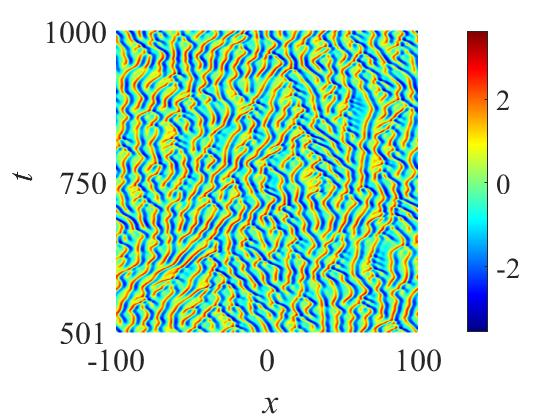
\includegraphics[width=.4\textwidth]{KS_result.jpg} 
%\end{center}
%\caption{KS方程式の結果}%図名
%\label{fig:ks}%fig図tb表
%\end{figure}

\newpage
\section{KS方程式のReservoir computingでの予測}
今回で用いた方程式は1D\ gKS方程式である.まず1D\ gKS方程式を下記に示す.
\begin{equation}
\frac{\partial u}{\partial t}+u\frac{\partial u}{\partial x}+\frac{\partial^2 u}{\partial x^2}+\delta\frac{\partial^3 u}{\partial x^3}+\nu\frac{\partial^4 u}{\partial x^4}=0
\label{eq:ks}
\end{equation}
今回のKS方程式でのパラメータを下記にまとめる.
\begin{itembox}[l]{KS方程式導出のパラメータ}
システムサイズ$L=-100\sim100$,刻み幅$dx=0.2$,刻み時間$dt=0.1$,時間$t=0\sim 10000$,$\delta=0$,$\nu=1.0$
\end{itembox}
\\
\ 次にスペクトル法によって導出されたKS方程式の解の最大値と最小値をそれぞれを$u_{max},u_{min}$とし,$-1\sim1$となるように入力正規化を行う.正規化された$u_{normal}$の導出方法を下記に示す.
\begin{equation}
u_{normal}=2\left(\frac{u-u_{min}}{u_{max}-u_{min}}-0.5\right)
\end{equation}
RCへと入力値を下記にまとめる.
\begin{itembox}[l]{入力されるKS方程式}
刻み幅$dx=1$ごとに並んだ入力値を用いる.\\
時間$dt=0.1$後を予測を行う.\\
入力値は$-1\sim1$に正規化された値を用いる.
\end{itembox}
\\
\ 最後にRCのパラメータを下記にまとめる.
\begin{itembox}[l]{RCのパラメータ}
学習回数97001回,初期のダイナミクスを除去するために最初の1000回は無視する.($t=0\sim100$)\\
出力回数1000回,入力層の数201個($L=-100\sim100$),出力層の数201個,中間層の数5000個\\
記憶力$\alpha=1.0$\\
入力層の重み$W_{in}$は,$-0.00258\sim0.00258$の一様分布\\
中間層の重み$W_{res}$は,$-0.000536\sim0.000536$の一様分布
\end{itembox}
\\
\ 以上のパラメータを用いて予測を行う.元の時系列データの$dt=0.1$刻みで$t=0\sim50$までの時空構造,RCで予測した出力の500回の時空構造,その2つの絶対誤差の時空構造の3つを下記に示す.
\begin{figure}[H]%[h]は記述したところ。[t]はそのページの上端。[t]はそのページの下端、[p]はページいっぱい
\begin{center}
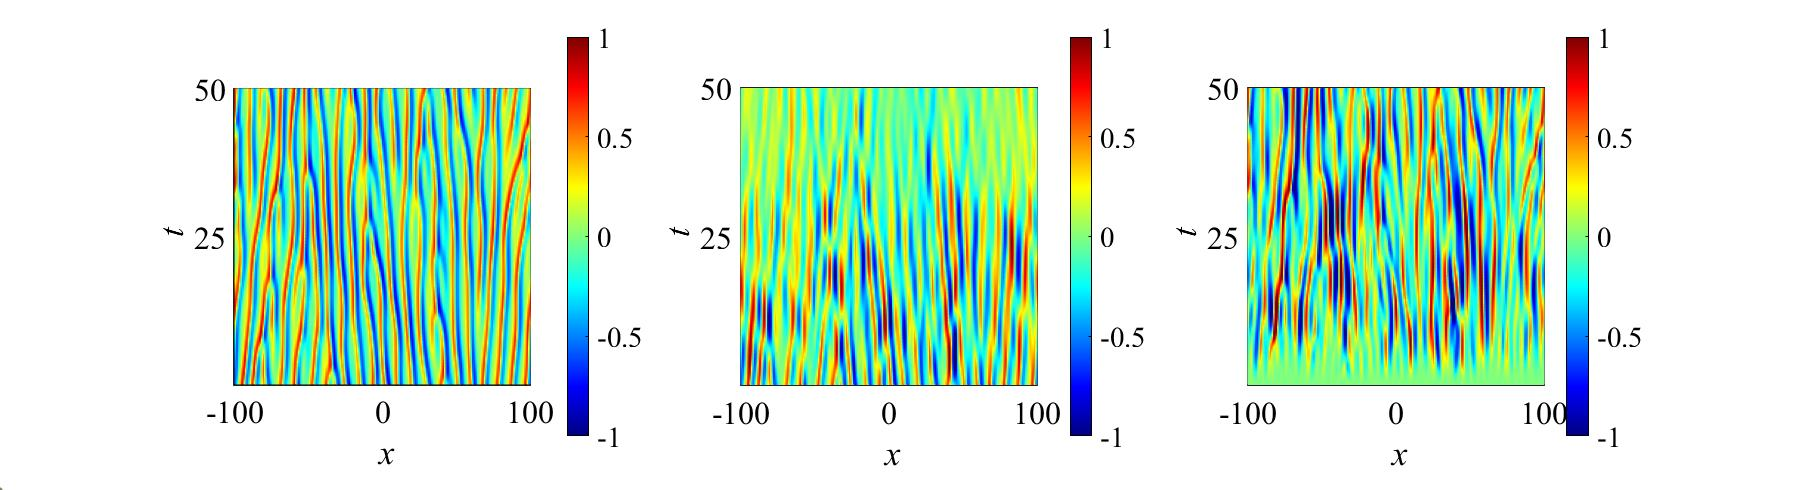
\includegraphics[width=.9\textwidth]{KS_error2.jpg} 
\end{center}
\caption{実際のKS方程式の時空構造(左図),RCで予測した時空構造(中央図),2つの絶対誤差の時空構造(右図)}%図名
\label{fig:KSRC}%fig図tb表
\end{figure}
この結果から時系列の50点($t=0\sim5$)程度までは予測ができていることがわかる.また,RCの予測結果は時間が経過するにつれて減衰してしまっていることがわかる.次に各位置における局所的な予測がうまくいっているのか確認するために,$L$の25刻みでの時間変化での元の時系列データとRCでの予測結果を示す.
\begin{figure}[H]%[h]は記述したところ。[t]はそのページの上端。[t]はそのページの下端、[p]はページいっぱい
\begin{center}
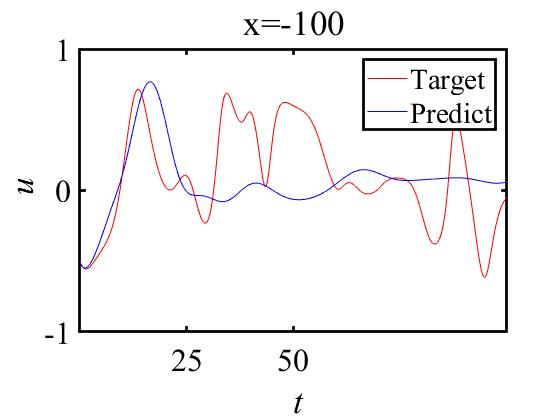
\includegraphics[width=.3\textwidth]{x=-100.jpg}
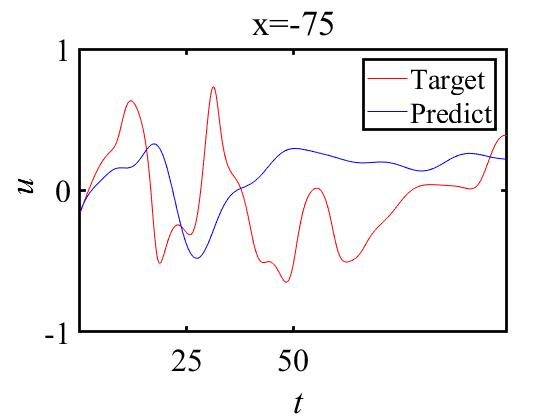
\includegraphics[width=.3\textwidth]{x=-75.jpg}
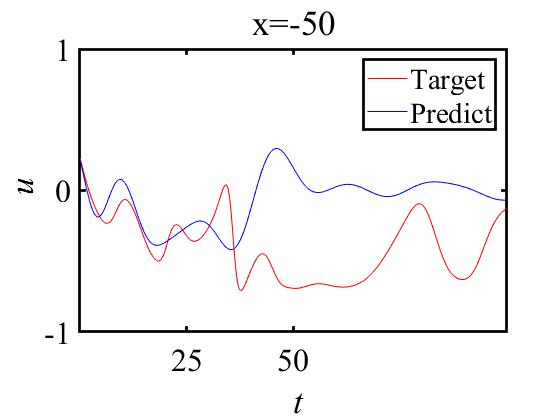
\includegraphics[width=.3\textwidth]{x=-50.jpg}
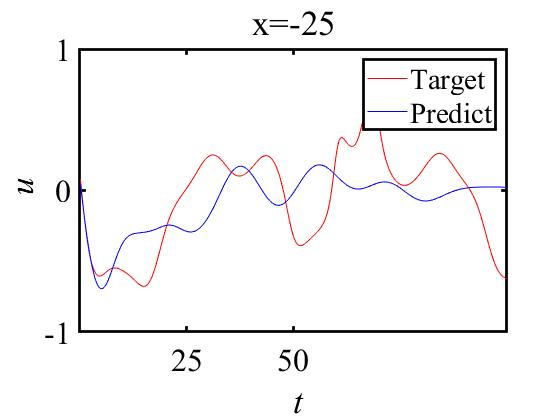
\includegraphics[width=.3\textwidth]{x=-25.jpg}
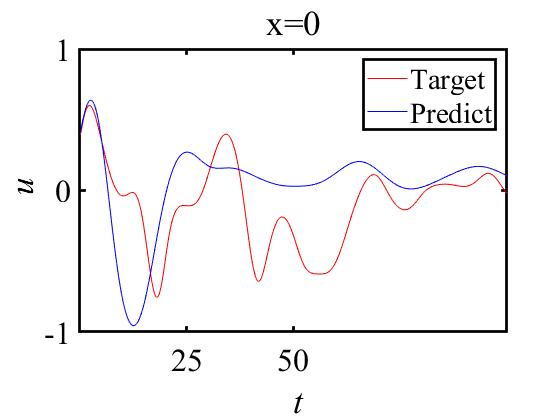
\includegraphics[width=.3\textwidth]{x=0.jpg}
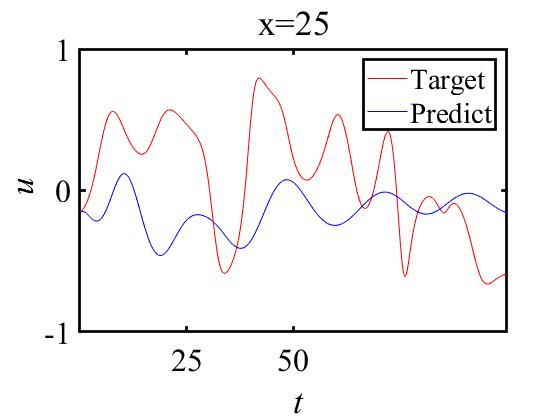
\includegraphics[width=.3\textwidth]{x=25.jpg}
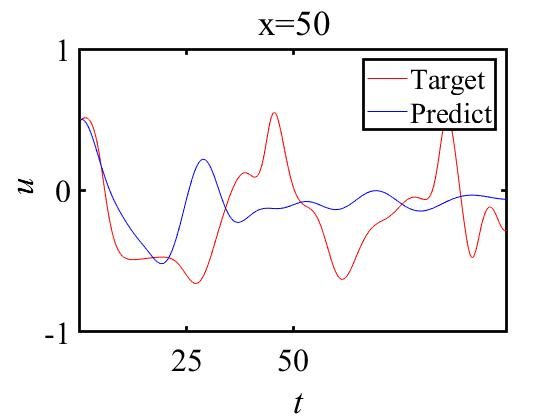
\includegraphics[width=.3\textwidth]{x=50.jpg}
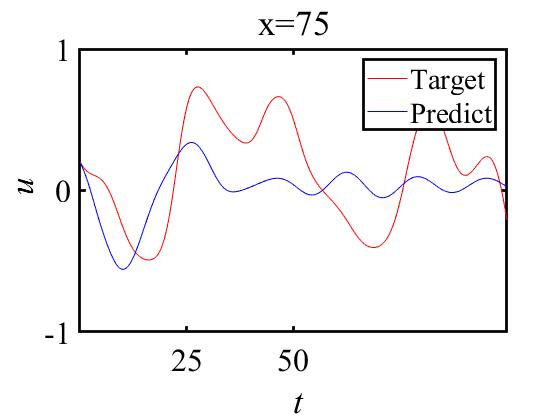
\includegraphics[width=.3\textwidth]{x=75.jpg}
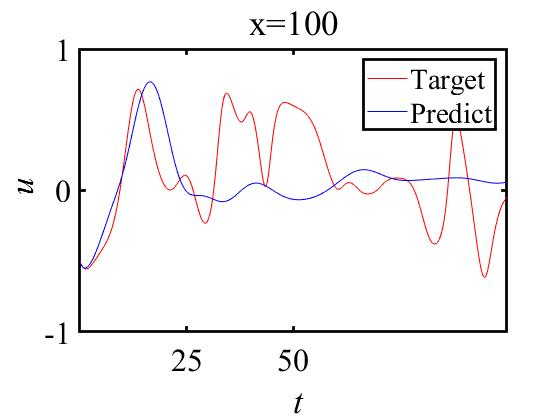
\includegraphics[width=.3\textwidth]{x=100.jpg}
\end{center}
\caption{$x$の25刻みごとの元の時系列と予測結果}%図名
\label{fig:x25}
\end{figure}
この結果からうまく予測できている位置とうまく予測できていない位置があることがわかる.予測がうまくいっている位置では,$t=0\sim20$の200点程度までは予測できていることがわかる.\\
\ 以上の結果から今後の課題として,より予測がうまくいくように学習数や中間層を大きくし予測の精度を上げる,$W_{in},W_{out}$の分布や値の範囲を変える,入力値の刻み幅,時間を変える,減衰してしまうことから$W_{out}$の行列の固有値が1より小さいことが考えられるので正方行列以外で固有値を求める方法を考え,実行する,入力値を最適な時間遅れさせた複数の値にするなどを行う必要がある.

\newpage
\section{今後の予定}
火炎のKS方程式の導出\\
\ or\\
\ スペクトル法\\
\ RCの改善


%\begin{figure}[H]%[h]は記述したところ。[t]はそのページの上端。[t]はそのページの下端、[p]はページいっぱい
%\begin{center}
%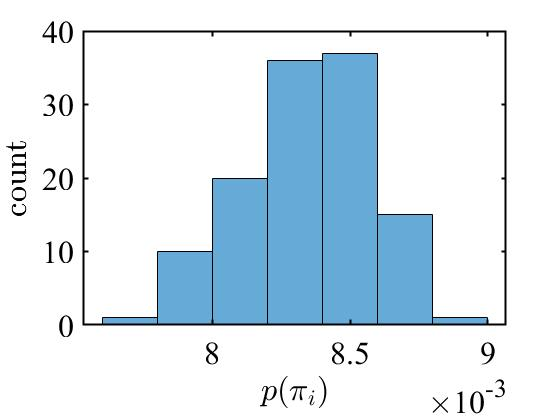
\includegraphics[width=.4\textwidth]{kadai3_histo.jpg}
%\end{center}
%\caption{課題3のヒストグラム(生成数は$100000$)}%図名
%\label{fig:kadai3_3}
%\end{figure}

%チェビシェフの不等式の置き換えの大数の弱法則から,
%\begin{equation}
%P(|\overline{X}_n-\mu|\ge \epsilon) \le \dfrac{\sigma^2}{n \epsilon^2}
%\end{equation}
%となる.ここでの$\overline{X}_n$はサンプルデータ$n$までの平均値(標本),$\mu$は理論的に考えられる平均値,$\epsilon$は許容誤差の大きさ,$\sigma$は標本データの分散である.




%$A^1$\cite{aaa}%参考文献



%\begin{itemize}
%\item アイテムコード1\\
%\item アイテムコード2\\
%\item アイテムコード3\\
%\item アイテムコード4\\
%\item アイテムコード5\\
%\end{itemize}


%\begin{figure}[H]%[h]は記述したところ。[t]はそのページの上端。[t]はそのページの下端、[p]はページいっぱい
%\begin{center}
%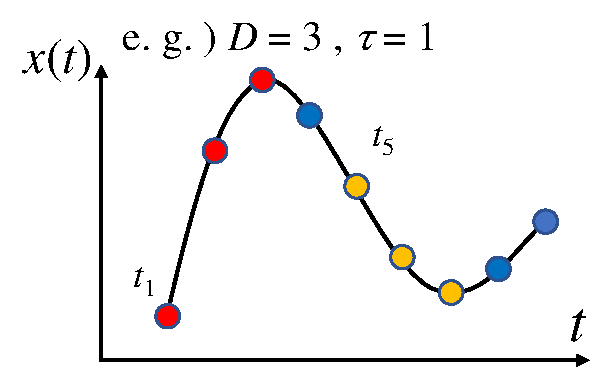
\includegraphics[width=.4\textwidth]{crop_PE1ver2.pdf} 
%\end{center}
%\caption{時系列$ x(t) $}%図名
%\label{fig:PE1}%fig図tb表
%\end{figure}

%\begin{eqnarray}
%\left\{%%{を作る
%\begin{array}{l}%l,llでは、lのときすべて{}の中の式のとき、{}の中にないものがあるならこっち
%\end{array}
%\right.
%\end{eqnarray} 

%式(8a)みたいなのができるぞ式の中で式番号振れるぞ
%\begin{subequations}
%\begin{align}
%a  &= b  & c  &= d  & e  &= f \label{eq:aaaa}\\
%a' &= b' & c' &= d' & e' &= f'\label{eq:bbbb}
%\end{align}
%\label{eq:cccc}
%\end{subequations}
%式(\ref{aaaa}),式(\ref{bbbb}),式(\ref{cccc})


\begin{thebibliography}{9999}%参考文献
\bibitem{all1}%参考文献citeするぞ
Erico L. Rempel, Abraham C.-L. Chian, Elbert E. N. Macau, and Reinaldo R. Rosa,"Analysis
of chaotic saddles in high-dimensional dynamical systems: The Kuramoto-Sivashinsky equation",
Chaos 14, 545 (2004).
\bibitem{all2}%参考文献citeするぞ
Aly-Khan Kassam,and Llotd N Treferhen,"FOURTH-ORDER TIME-STEPPING FOR STIFF
PDEs", SIAM J. SCI. COMPUT. Vol. 26, No. 4, pp.1214$\sim$1233(2005).
%\bibitem{re}
%カオス・フラクタル\ 講義ノート\ \#8,\url{https://ocw.hokudai.ac.jp/wp-content/uploads/2016/01/ChaosFractal-2011-Note-08.pdf}
%\bibitem{wgn}%参考文献citeするぞ
%ホワイトガウスノイズサンプルの生成-MATLAD wgn,\url{https://jp.mathworks.com/help/comm/ref/wgn.html}
%\bibitem{mutual}
%相互情報量の意味とエントロピーとの関係 | 高校数学の美しい物語,\url{https://mathtrain.jp/mutualinfo}
%\bibitem{net}
%複雑ネットワーク:統計物理学の視点,\url{http://mercury.yukawa.kyoto-u.ac.jp/~bussei.kenkyu/pdf/03/1/9999-031210.pdf}
\end{thebibliography}

%\newpage



\end{document}